\section{Introduction}
\subsection{Community Structure Identification Problem}
The Community Structure Identification Problem is a fundamental challenge in network analysis and graph theory. It involves identifying groups or communities within a given network where nodes within the same community are densely connected to each other while having fewer connections to nodes in other communities.

The problem arises in various real-world scenarios, such as social networks, biological networks, and online communities. By uncovering the underlying community structure, researchers can gain valuable insights into the organization, dynamics, and functionality of complex systems.

Solving the Community Structure Identification Problem typically entails applying graph clustering algorithms to partition the network into cohesive communities. These algorithms aim to maximize the modularity, a measure that quantifies the quality of the community structure by comparing the observed connections within communities to those expected by chance.

Some example: 
\begin{itemize}
\item\textbf{Social Networks: }Consider a social network platform like Facebook or Twitter. The problem involves identifying distinct groups or communities of users who share similar interests, have common social connections, or engage in similar discussions. By identifying these communities, the platform can better understand user behavior, personalize content recommendations, and detect influential users or potential communities of interest.
% \subsubsection{Modularity Q}
\item\textbf{Biological Networks:} In molecular biology, the problem arises in analyzing protein-protein interaction networks or gene co-expression networks. Identifying communities within these networks can reveal groups of proteins or genes that work together to perform specific biological functions or participate in shared signaling pathways. This knowledge can aid in understanding disease mechanisms, drug discovery, and the design of targeted therapies.
\item\textbf{Online Communities:} In online forums, discussion boards, or social media platforms, the Community Structure Identification Problem involves identifying clusters of users who interact and engage with each other on specific topics or interests. Uncovering these communities can help in moderating online discussions, identifying influential users, and facilitating content recommendation or targeted advertising.
\item\textbf{Citation Networks:} In academic research, the problem arises in analyzing citation networks, where papers cite other papers. By identifying communities within these networks, researchers can discover clusters of related papers that contribute to specific research topics or subfields. This information can aid in literature review, knowledge discovery, and identifying potential collaborators or experts in a particular domain.
\item\textbf{Transportation Networks:} In transportation planning and optimization, the problem involves identifying communities or clusters of interconnected transportation hubs, such as airports or railway stations. By identifying these communities, transportation authorities can optimize routing, improve connectivity, and identify potential bottlenecks or areas for infrastructure development
\end{itemize}

\begin{center}
\begin{figure}[!htp]
    \centering
    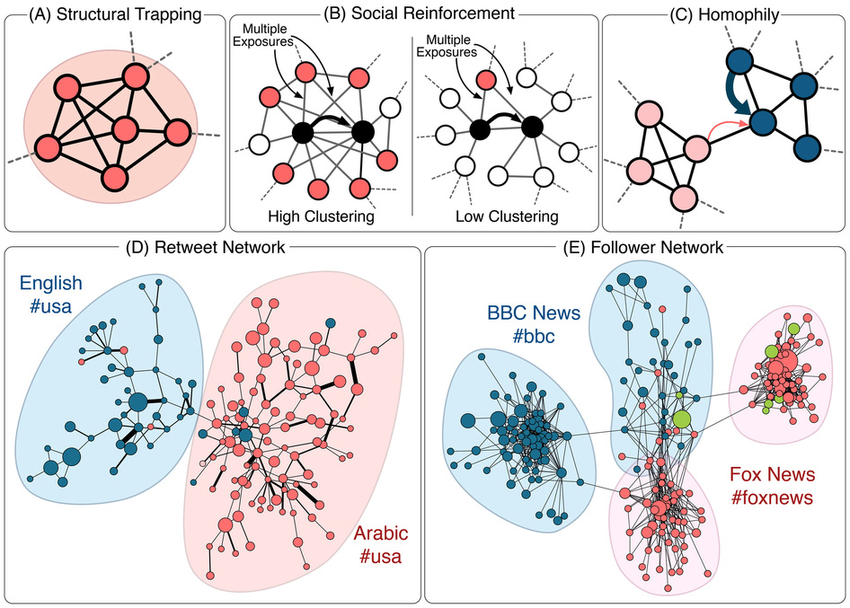
\includegraphics[width=0.8 \textwidth]{image/SocialNetworkApplicated.png}
    \caption{The importance of community structure in the spreading of social contagions}
    \label{subsection}
\end{figure}
\end{center}

\subsection{Community Structure Identification for book}
\subsubsection{Motivation}
Consider a network where each node represents a book, and the connections between nodes represent similarities or relationships between books. These relationships can be based on various factors such as genre, author, themes, or even reader reviews and recommendations.

\begin{center}
\begin{figure}[!htp]
    \centering
    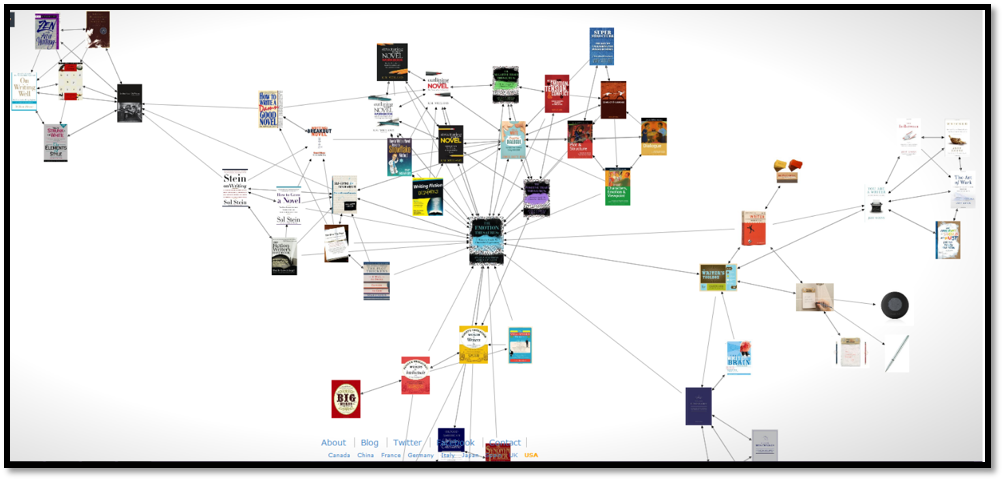
\includegraphics[width=1 \textwidth]{image/BookNetwork.png}
    \caption{Book network example}
    \label{subsection}
\end{figure}
\end{center}\

The Community Structure Identification Problem in this scenario involves identifying clusters of books that share common characteristics, themes, or appeal to similar audiences. By uncovering these book communities, we can gain insights into the organization of the literary landscape and identify groups of books that are related in terms of content, style, or target readership.

For instance, the algorithm might identify a community of classic literature, consisting of books by authors such as Jane Austen, Charles Dickens, and F. Scott Fitzgerald. Another community might comprise contemporary romance novels by popular authors like Nicholas Sparks and Jojo Moyes. The nodes within these communities would be densely connected, indicating strong similarities between the books within each community.

This information can be valuable for various stakeholders in the book industry. Publishers can identify potential target markets and optimize their marketing strategies by understanding which communities of books are likely to appeal to similar readers. Online book retailers can enhance recommendation systems by suggesting books from the same community or providing "read-alike" recommendations to customers. Authors can gain insights into their genre or niche and better understand their position within the broader literary landscape.

In summary, the Community Structure Identification Problem in the context of books helps reveal clusters of books that share common attributes, themes, or readership, enabling targeted marketing, recommendation systems, and a deeper understanding of the literary world.

\subsubsection{Dataset description}

\textbf{Context}: Books read by users and ratings provided by them on Amazon

\textbf{Content}: Online data for books from Amazon along with user ratings and users who bought them. Totaly 3 files:
\begin{itemize}
    \item Books.csv -> Has the book descescription, include some fields: 
    \begin{enumerate}
        \item Book ID: 10 digit number, ID of the book (unique value).
        \item Title: free text, title of the book. 
        \item Author: free text, book author name.
        \item Publish year: number, the year that book published. 
        \item Publisher: free text, the publisher name.
        \item Images: free text, link to image of the book.
    \end{enumerate}
    \item Ratings.csv -> Has the book ratings description, include some fields: 
    \begin{enumerate}
        \item User ID: 6 digit number, ID of the user.
        \item Book ID: 10 digit number, ID of the book.
        \item Book rating from user: number from 0 to 10, rating score from user to the book. 
    \end{enumerate}
    \item Users.csv -> Has the user descriptions, include some fields: 
    \begin{enumerate}
        \item User ID: 6 digit number, ID of the user.
        \item Location: free text, location of the user.
        \item Age: number, user age.
    \end{enumerate}
\end{itemize}


